\section{Elementos do circuito pneumático e exemplos básicos}


\begin{frame}{Introdução}
\begin{block}{Elementos do sistema}
	Um circuito pneumático é composto por muitas partes.
	\begin{itemize}
		\item Uma ``fonte de energia'' (unidade de condicionamento).
		\item Elementos de sinal.
		\item Elementos de processamento de sinal.
		\item Elementos de comando.
		\item Elementos de trabalho.
	\end{itemize}
\end{block}
\end{frame}


\begin{frame}{Introdução}
	\centering
	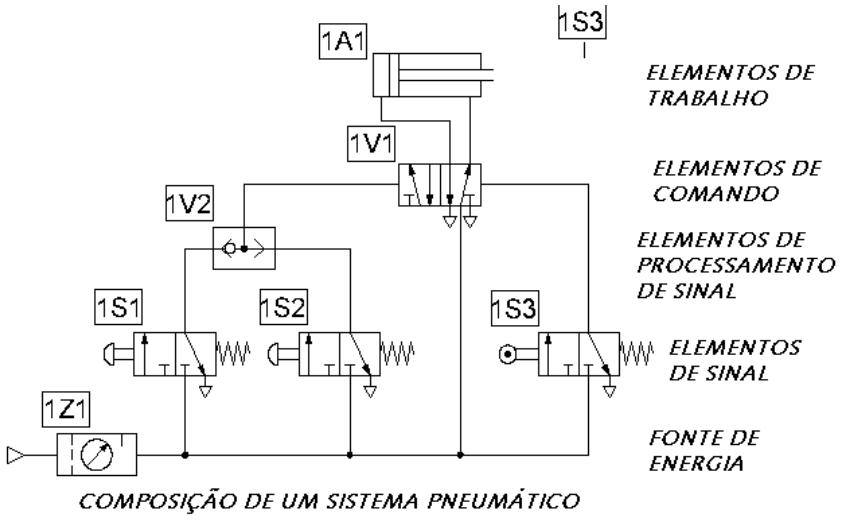
\includegraphics[width=0.9\linewidth]{Figuras/Ch14/fig01}
	
	Diagrama de circuito pneumático
\end{frame}


\begin{frame}{Introdução}
\begin{block}{Unidade de condicionamento}
	\begin{itemize}
		\item A unidade de condicionamento já foi abordada anteriormente, e é nela que começa todo circuito pneumático, por ser a fonte de ar comprimido.
		\item Possui duas simbologias:
	\end{itemize}
\end{block}

\begin{minipage}[c]{0.45\linewidth}
	\centering
	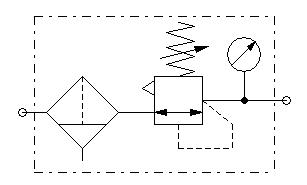
\includegraphics[width=1\linewidth]{Figuras/Ch14/fig02}
	
	Representação integral
\end{minipage}
\hfill
\begin{minipage}[c]{0.45\linewidth}
	\centering
	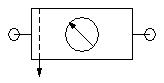
\includegraphics[width=1\linewidth]{Figuras/Ch14/fig03}
	
	Representação simplificada (mais comum)
\end{minipage}
\end{frame}


\begin{frame}{Elementos de sinal - Válvulas de controle direcional}
	\begin{block}{Introdução}
		Existem vários modelos de \textbf{válvulas de controle direcional}, sendo necessário identificá-las e reconhecer suas principais diferenças.
		
		\smallskip
		
		Uma válvula de controle direcional é identificada a partir de algumas variáveis:
		\begin{itemize}
			\item Posição inicial.
			\item Número de posições.
			\item Número de vias.
			\item Tipo de acionamento.
			\item Tipo de retorno.
		\end{itemize}
	\end{block}
\end{frame}


\begin{frame}{Elementos de sinal - Válvulas de controle direcional}
	\begin{block}{Número de posições}
		Pode ser determinado observando o desenho da válvula:
	\end{block}

	\medskip

	\centering
		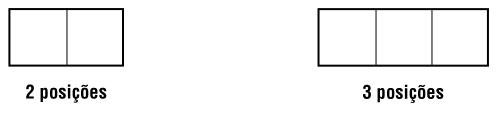
\includegraphics[width=0.7\linewidth]{Figuras/Ch14/fig04}
		
	\medskip
	
	\begin{block}{}
		\begin{itemize}
			\item Basta contar por \textbf{quantos quadradinhos é composta}, isso nos dirá quantas posições possui.
			\item A quantidade de posições nos informa as possibilidades de manobra dessa válvula, isto é, o que podemos fazer com ela.
		\end{itemize}
	\end{block}
\end{frame}


\begin{frame}{Elementos de sinal - Válvulas de controle direcional}
	\begin{block}{Número de vias}
		Devemos contar a \textbf{quantidade de pontos onde o desenho interior da válvula toca suas bordas} (superior e inferior).
	\end{block}
	
	\medskip
	
	\centering
	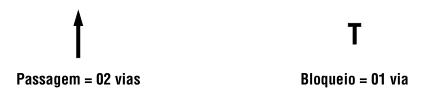
\includegraphics[width=0.7\linewidth]{Figuras/Ch14/fig05}
	
	\medskip
	
	\begin{block}{}
		\begin{itemize}
			\item Os possíveis desenhos são as \textbf{setas} e os \textbf{T}'s.
			\item As \textbf{setas} representam passagens de fluxo, mas não necessariamente seu sentido.
			\item Os \textbf{T}'s representam um bloqueio do fluxo.
		\end{itemize}
	\end{block}
\end{frame}


\begin{frame}{Elementos de sinal - Válvulas de controle direcional}
	\centering
	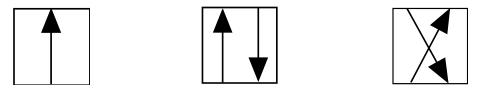
\includegraphics[width=0.87\linewidth]{Figuras/Ch14/fig06}
	
	\medskip
	
	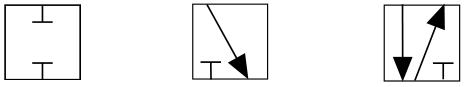
\includegraphics[width=0.85\linewidth]{Figuras/Ch14/fig07}
	
	\medskip
	
	Exemplos de utilização dos símbolos de fluxo
\end{frame}


\begin{frame}{Elementos de sinal - Válvulas de controle direcional}
	\begin{block}{Nomeando válvulas - Exemplo \#01}
		\begin{itemize}
			\item A nomenclatura mais elementar em relação às válvulas é quanto às suas \textbf{posições} e \textbf{número de vias}.
			\item Uma válvula que tem \textbf{três vias }e \textbf{duas posições }é conhecida como ``3/2 vias'' (lê-se ``três duas vias'').
		\end{itemize}
	\end{block}
	
	\medskip
	
	\centering
	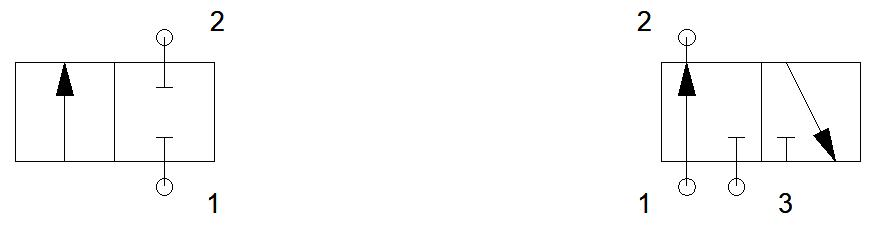
\includegraphics[width=0.9\linewidth]{Figuras/Ch14/fig08}
	
	Exemplos de válvulas reais simplificadas
\end{frame}


\begin{frame}{Elementos de sinal - Válvulas de controle direcional}
	\begin{block}{Numerando vias}
		Havendo múltiplas vias em toda válvula, é útil que se faça alguma forma de \textbf{identificação}. Para isso existe um sistema de \textbf{numeração das vias} das válvulas de controle direcional.
		\begin{itemize}
			\item A via número 1 é \textbf{sempre} a \textbf{alimentação de ar comprimido} da válvula.
			\item Números pares (2,4) são usados para \textbf{utilização} ou \textbf{saída} de ar comprimido.
			\item Números ímpares após o 1 (3,5) são usados para \textbf{escape} ou \textbf{exaustão} de ar comprimido.
		\end{itemize}
	\end{block}
\end{frame}


\begin{frame}{Elementos de sinal - Válvulas de controle direcional}
	\begin{block}{Acionamento}
		Existem muitas formas de acionar as válvulas de controle direcional, por isso são divididos em \textbf{quatro} categorias principais:
		\begin{itemize}
			\item Musculares.
			\item Mecânicos.
			\item Pneumáticos.
			\item Elétricos.
		\end{itemize}
	\end{block}
\end{frame}


\begin{frame}{Elementos de sinal - Válvulas de controle direcional}
	\begin{minipage}[c]{0.48\linewidth}
		\centering
		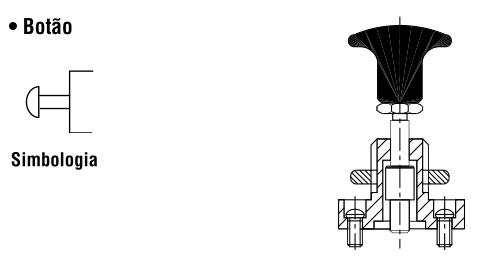
\includegraphics[width=1\linewidth]{Figuras/Ch14/fig09}
	\end{minipage}
	\hfill
	\begin{minipage}[c]{0.48\linewidth}
		\centering
		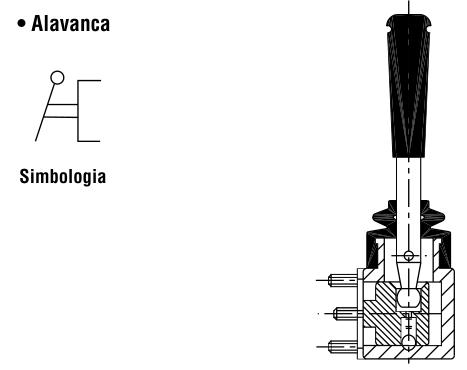
\includegraphics[width=1\linewidth]{Figuras/Ch14/fig10}
	\end{minipage}

	\centering
	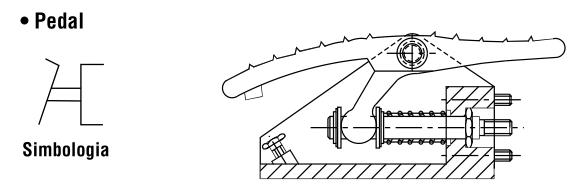
\includegraphics[width=0.5\linewidth]{Figuras/Ch14/fig11}
	
	\medskip
	
	Acionamento muscular
\end{frame}


\begin{frame}{Elementos de sinal - Válvulas de controle direcional}
	\begin{minipage}[c]{0.48\linewidth}
		\centering
		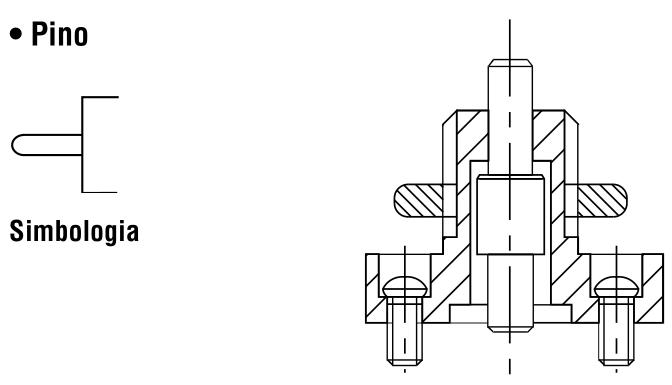
\includegraphics[width=1\linewidth]{Figuras/Ch14/fig12}
	\end{minipage}
	\hfill
	\begin{minipage}[c]{0.48\linewidth}
		\centering
		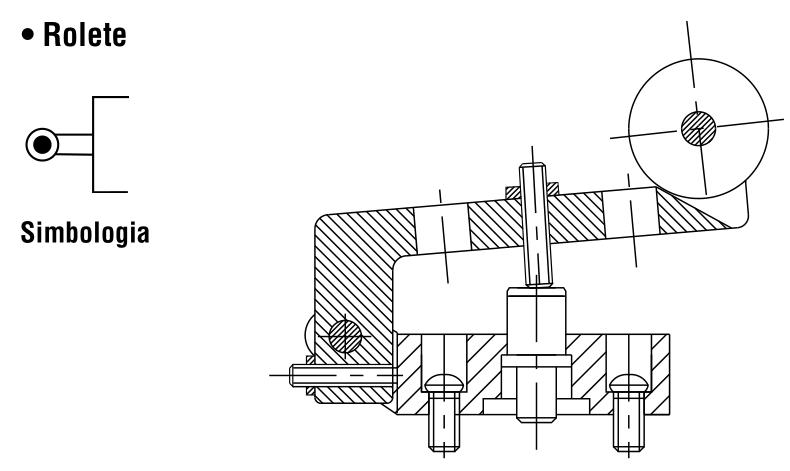
\includegraphics[width=1\linewidth]{Figuras/Ch14/fig13}
	\end{minipage}
	
	\centering
	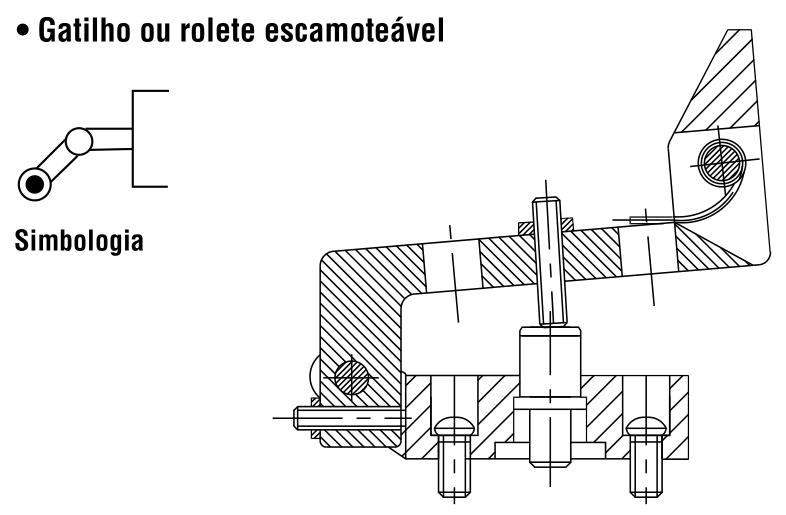
\includegraphics[width=0.4\linewidth]{Figuras/Ch14/fig14}
	
	\medskip
	
	Acionamento mecânico
\end{frame}


\begin{frame}{Elementos de sinal - Válvulas de controle direcional}
	\begin{minipage}[c]{0.48\linewidth}
		\centering
		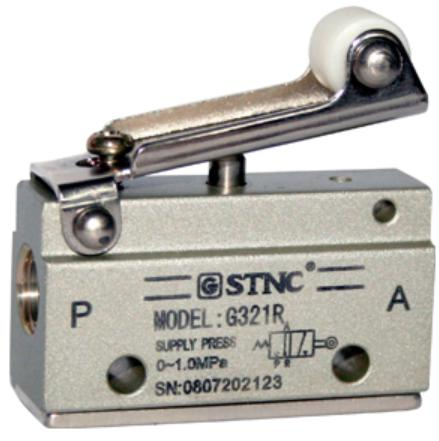
\includegraphics[width=0.9\linewidth]{Figuras/Ch14/fig15}
		
		Rolete
	\end{minipage}
	\hfill
	\begin{minipage}[c]{0.48\linewidth}
		\centering
		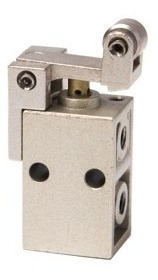
\includegraphics[height=0.7\textheight]{Figuras/Ch14/fig16}
		
		Rolete escamoteável
	\end{minipage}

	\centering
	\bigskip
	
	Acionamento mecânico
\end{frame}


\begin{frame}{Elementos de sinal - Válvulas de controle direcional}
	\begin{minipage}[c]{0.48\linewidth}
		\centering
		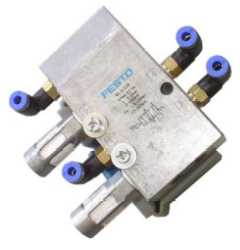
\includegraphics[width=0.9\linewidth]{Figuras/Ch14/fig17}
		
		\medskip
		
		Acionamento pneumático
	\end{minipage}
	\hfill
	\begin{minipage}[c]{0.48\linewidth}
		\centering
		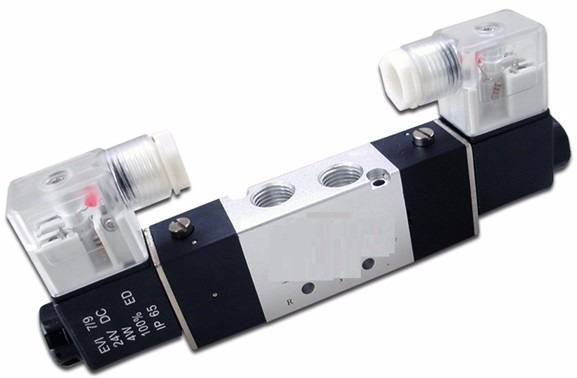
\includegraphics[width=1\linewidth]{Figuras/Ch14/fig18}
		
		\bigskip
		
		Acionamento por solenoide
	\end{minipage}
\end{frame}


\begin{frame}{Elementos de sinal - Válvulas de controle direcional}
	\begin{block}{Posição inicial}
		\begin{itemize}
			\item A posição inicial da válvula é indicada pela posição ``central'' em sua representação, isto é, a posição onde as entradas e saídas \textbf{permanecem }no caso de a válvula \textbf{não }ter sido \textbf{atuada}.
			\item Uma válvula de duas posições pode ser NA ou NF, isto é, \textit{Normal Aberta }ou \textit{Normal Fechada}.
			\item Ao contrário dos contatos em acionamentos elétricos, as válvulas pneumáticas são ditas \textbf{normalmente abertas}, se \textbf{permitem} a passagem de fluxo, e \textbf{normalmente fechadas} se \textbf{restringem} essa passagem.
		\end{itemize}
	\end{block}
\end{frame}


\begin{frame}{Elementos de sinal - Válvulas de controle direcional}
	
	\centering
	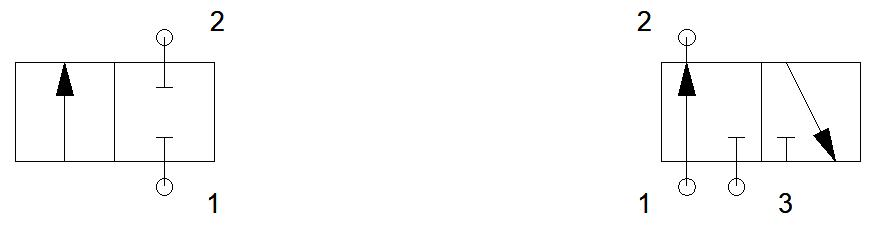
\includegraphics[width=0.9\linewidth]{Figuras/Ch14/fig08}
	
	\medskip
	
	Exemplos de válvulas reais simplificadas
\end{frame}


\begin{frame}{Elementos de sinal - Válvulas de controle direcional}
	\begin{block}{Nomeando válvulas - Exemplo \#02}
		\begin{itemize}
			\item Depois do número de posições e vias devemos informar a posição inicial (NA ou NF) e também o tipo de acionamento.
		\end{itemize}
	\end{block}
	
	\medskip
	
	\begin{minipage}[c]{0.48\linewidth}
		\centering
		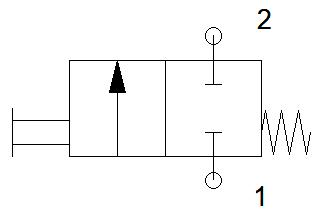
\includegraphics[width=1\linewidth]{Figuras/Ch14/fig19}
	\end{minipage}
	\hfill
	\begin{minipage}[c]{0.48\linewidth}
		\centering
		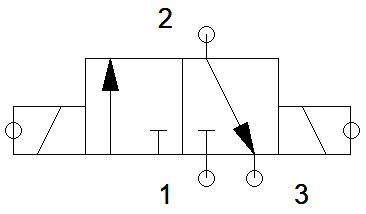
\includegraphics[width=1\linewidth]{Figuras/Ch14/fig20}
	\end{minipage}

	\centering
	\medskip
	
	Exemplos de válvulas reais
\end{frame}


\begin{frame}{Elementos de processamento de sinais - Válvulas auxiliares}
	\begin{block}{Introdução}
		\begin{itemize}
			\item As válvulas auxiliares realizam funções lógicas no circuito pneumático.
		\end{itemize}
	\end{block}

	\medskip
	
	\centering
	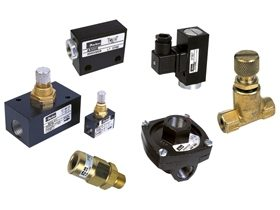
\includegraphics[width=0.7\linewidth]{Figuras/Ch14/fig20n2}
	
\end{frame}


\begin{frame}{Elementos de processamento de sinais - Válvulas auxiliares}
	\begin{block}{Válvula de retenção}
		\begin{itemize}
			\item Garante o sentido do fluxo.
		\end{itemize}
	\end{block}

	\medskip
	
	\begin{minipage}[c]{0.48\linewidth}
		\centering
		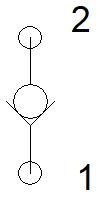
\includegraphics[height=0.7\textheight]{Figuras/Ch14/fig21}
	\end{minipage}
	\hfill
	\begin{minipage}[c]{0.48\linewidth}
		\centering
		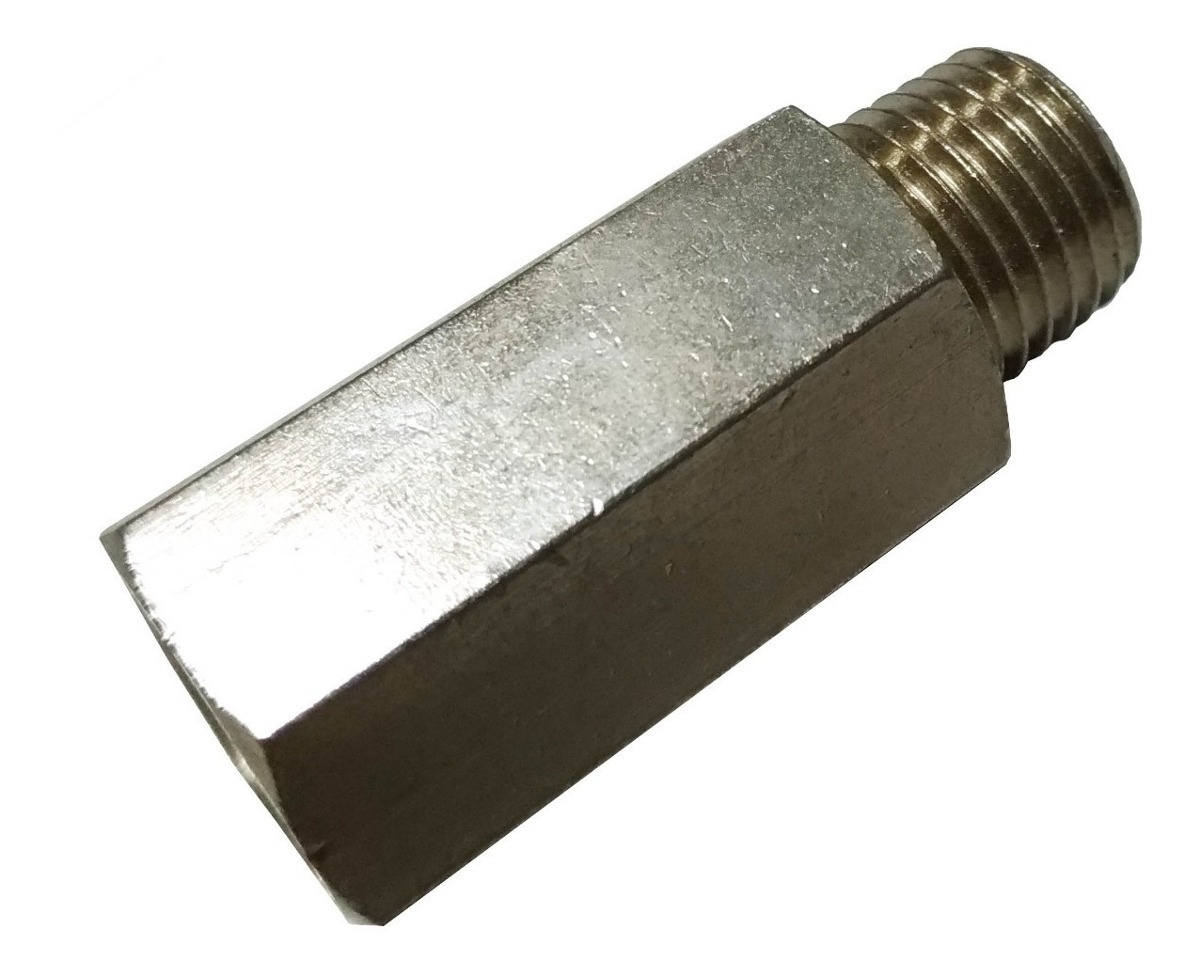
\includegraphics[width=1\linewidth]{Figuras/Ch14/fig22}
	\end{minipage}
\end{frame}


\begin{frame}{Elementos de processamento de sinais - Válvulas auxiliares}
	\begin{block}{Elemento OU}
		\begin{itemize}
			\item Realiza a função lógica OU entre duas entradas.
		\end{itemize}
	\end{block}
	
	\medskip
	
	\begin{minipage}[c]{0.48\linewidth}
		\centering
		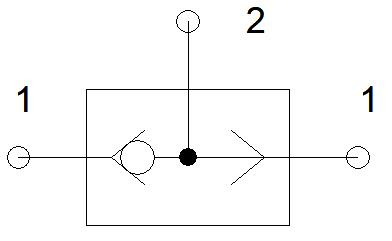
\includegraphics[width=1\linewidth]{Figuras/Ch14/fig23}
	\end{minipage}
	\hfill
	\begin{minipage}[c]{0.48\linewidth}
		\centering
		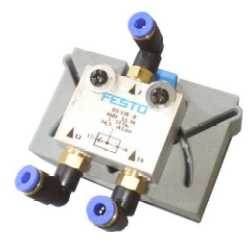
\includegraphics[width=1\linewidth]{Figuras/Ch14/fig24}
	\end{minipage}
\end{frame}


\begin{frame}{Elementos de processamento de sinais - Válvulas auxiliares}
	\begin{block}{Elemento E}
		\begin{itemize}
			\item Realiza a função lógica E entre duas entradas.
		\end{itemize}
	\end{block}
	
	\medskip
	
	\begin{minipage}[c]{0.48\linewidth}
		\centering
		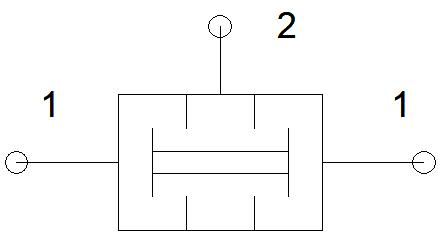
\includegraphics[width=1\linewidth]{Figuras/Ch14/fig25}
	\end{minipage}
	\hfill
	\begin{minipage}[c]{0.48\linewidth}
		\centering
		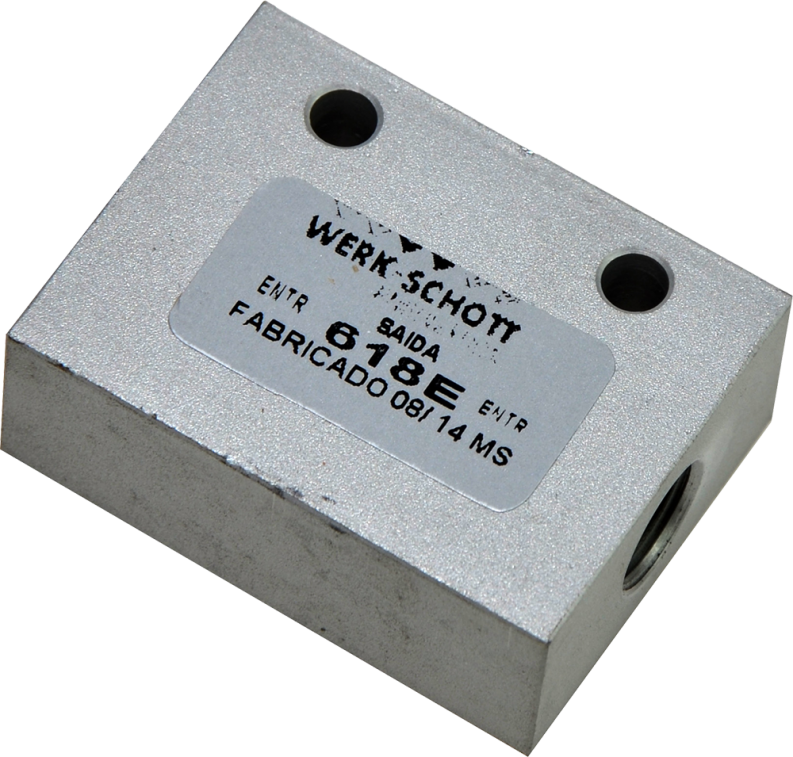
\includegraphics[width=1\linewidth]{Figuras/Ch14/fig26}
	\end{minipage}
\end{frame}


\begin{frame}{Elementos de processamento de sinais - Válvulas auxiliares}
	\begin{block}{Válvula de controle de fluxo}
		\begin{itemize}
			\item Controla a quantidade de fluxo de ar comprimido.
		\end{itemize}
	\end{block}
	
	\medskip
	
	\begin{minipage}[c]{0.48\linewidth}
		\centering
		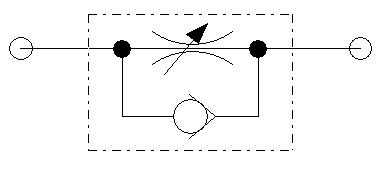
\includegraphics[width=1\linewidth]{Figuras/Ch14/fig27}
	\end{minipage}
	\hfill
	\begin{minipage}[c]{0.48\linewidth}
		\centering
		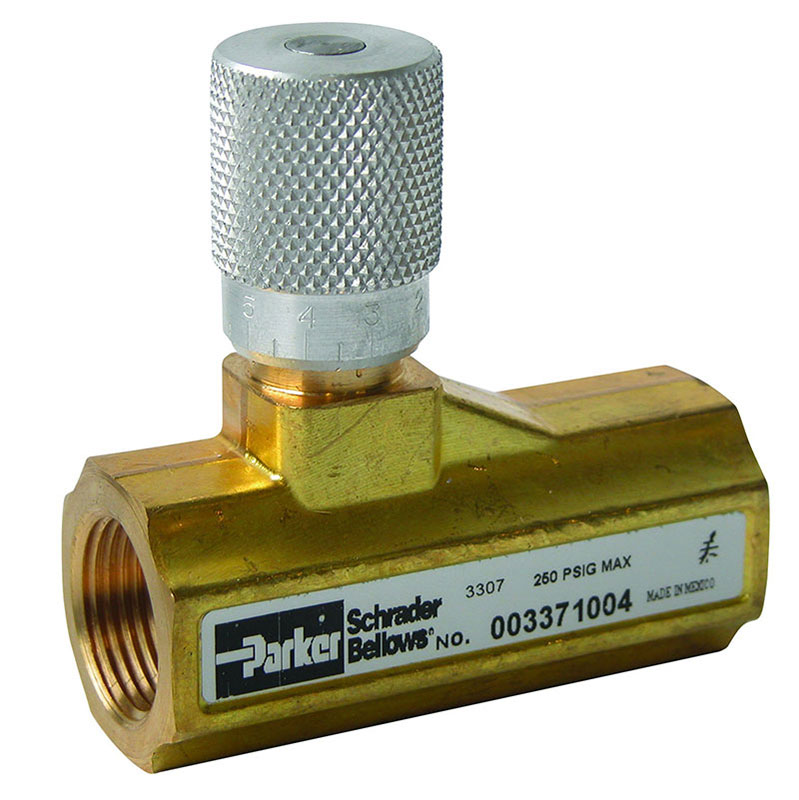
\includegraphics[width=1\linewidth]{Figuras/Ch14/fig28}
	\end{minipage}
\end{frame}


\begin{frame}{Elementos de comando}
	\begin{block}{Válvulas de controle direcional}
		Os elementos de comando são os mesmos dos elementos de sinal, porém diferem em uso:
		\begin{itemize}
			\item Os \textbf{elementos de sinal} são usados para captar sinais úteis do processo ou de um operador.
			\item Os \textbf{elementos de comando} são usados para comandar os \textbf{elementos de trabalho}.
		\end{itemize}
	\end{block}
\end{frame}


\begin{frame}{Elementos de trabalho - Atuadores pneumáticos}
	\begin{block}{Introdução}
		\begin{itemize}
			\item A energia pneumática é transformada em movimento e força através dos elementos de trabalho.
			\item Esses movimentos podem ser lineares ou rotativos.
			\item Os movimentos lineares são executados pelos cilindros e os movimentos rotativos pelos rotores pneumáticos e cilindros rotativos.
		\end{itemize}
	\end{block}

	\medskip
	
	\centering
	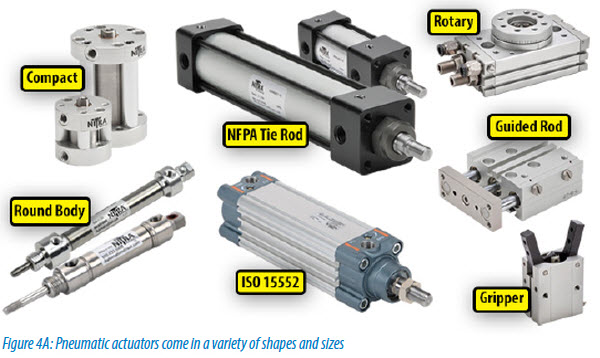
\includegraphics[width=0.6\linewidth]{Figuras/Ch14/fig29}
	
\end{frame}


\begin{frame}{Elementos de trabalho - Atuadores pneumáticos}
	\begin{block}{Cilindros pneumáticos}
		\begin{itemize}
			\item Cilindro de simples ação.
			\item Cilindro de dupla ação.
		\end{itemize}
	\end{block}
	
	\medskip
	
	\centering
	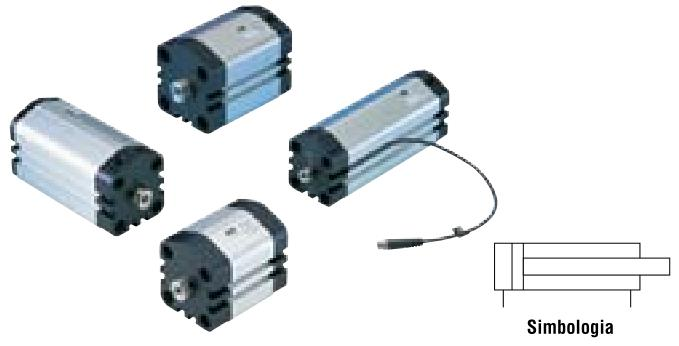
\includegraphics[width=0.7\linewidth]{Figuras/Ch14/fig30}
	
\end{frame}


\begin{frame}{Elementos de trabalho - Atuadores pneumáticos}
	\begin{block}{Cilindro de simples ação}
		\begin{itemize}
			\item Recebe ar somente de um lado.
		\end{itemize}
	\end{block}
	
	\medskip
	
	\begin{minipage}[c]{0.48\linewidth}
		\centering
		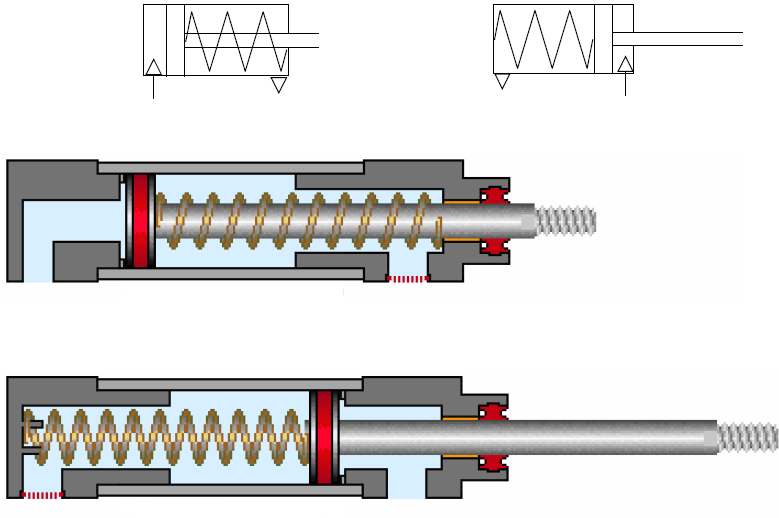
\includegraphics[width=1\linewidth]{Figuras/Ch14/fig31}
	\end{minipage}
	\hfill
	\begin{minipage}[c]{0.48\linewidth}
		\centering
		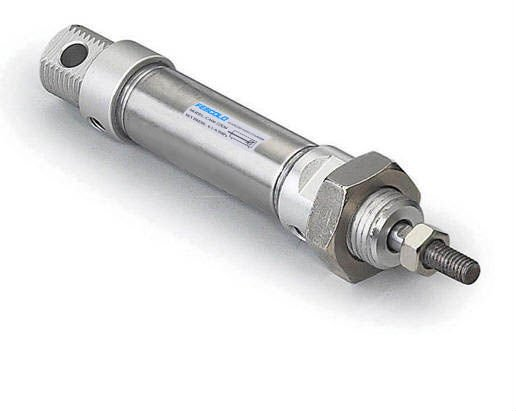
\includegraphics[width=1\linewidth]{Figuras/Ch14/fig32}
	\end{minipage}
	
\end{frame}


\begin{frame}{Elementos de trabalho - Atuadores pneumáticos}
	\begin{block}{Cilindro de dupla ação}
		\begin{itemize}
			\item Recebe ar dos dois lados.
		\end{itemize}
	\end{block}

	\medskip
	
	\begin{minipage}[c]{0.38\linewidth}
		\centering
		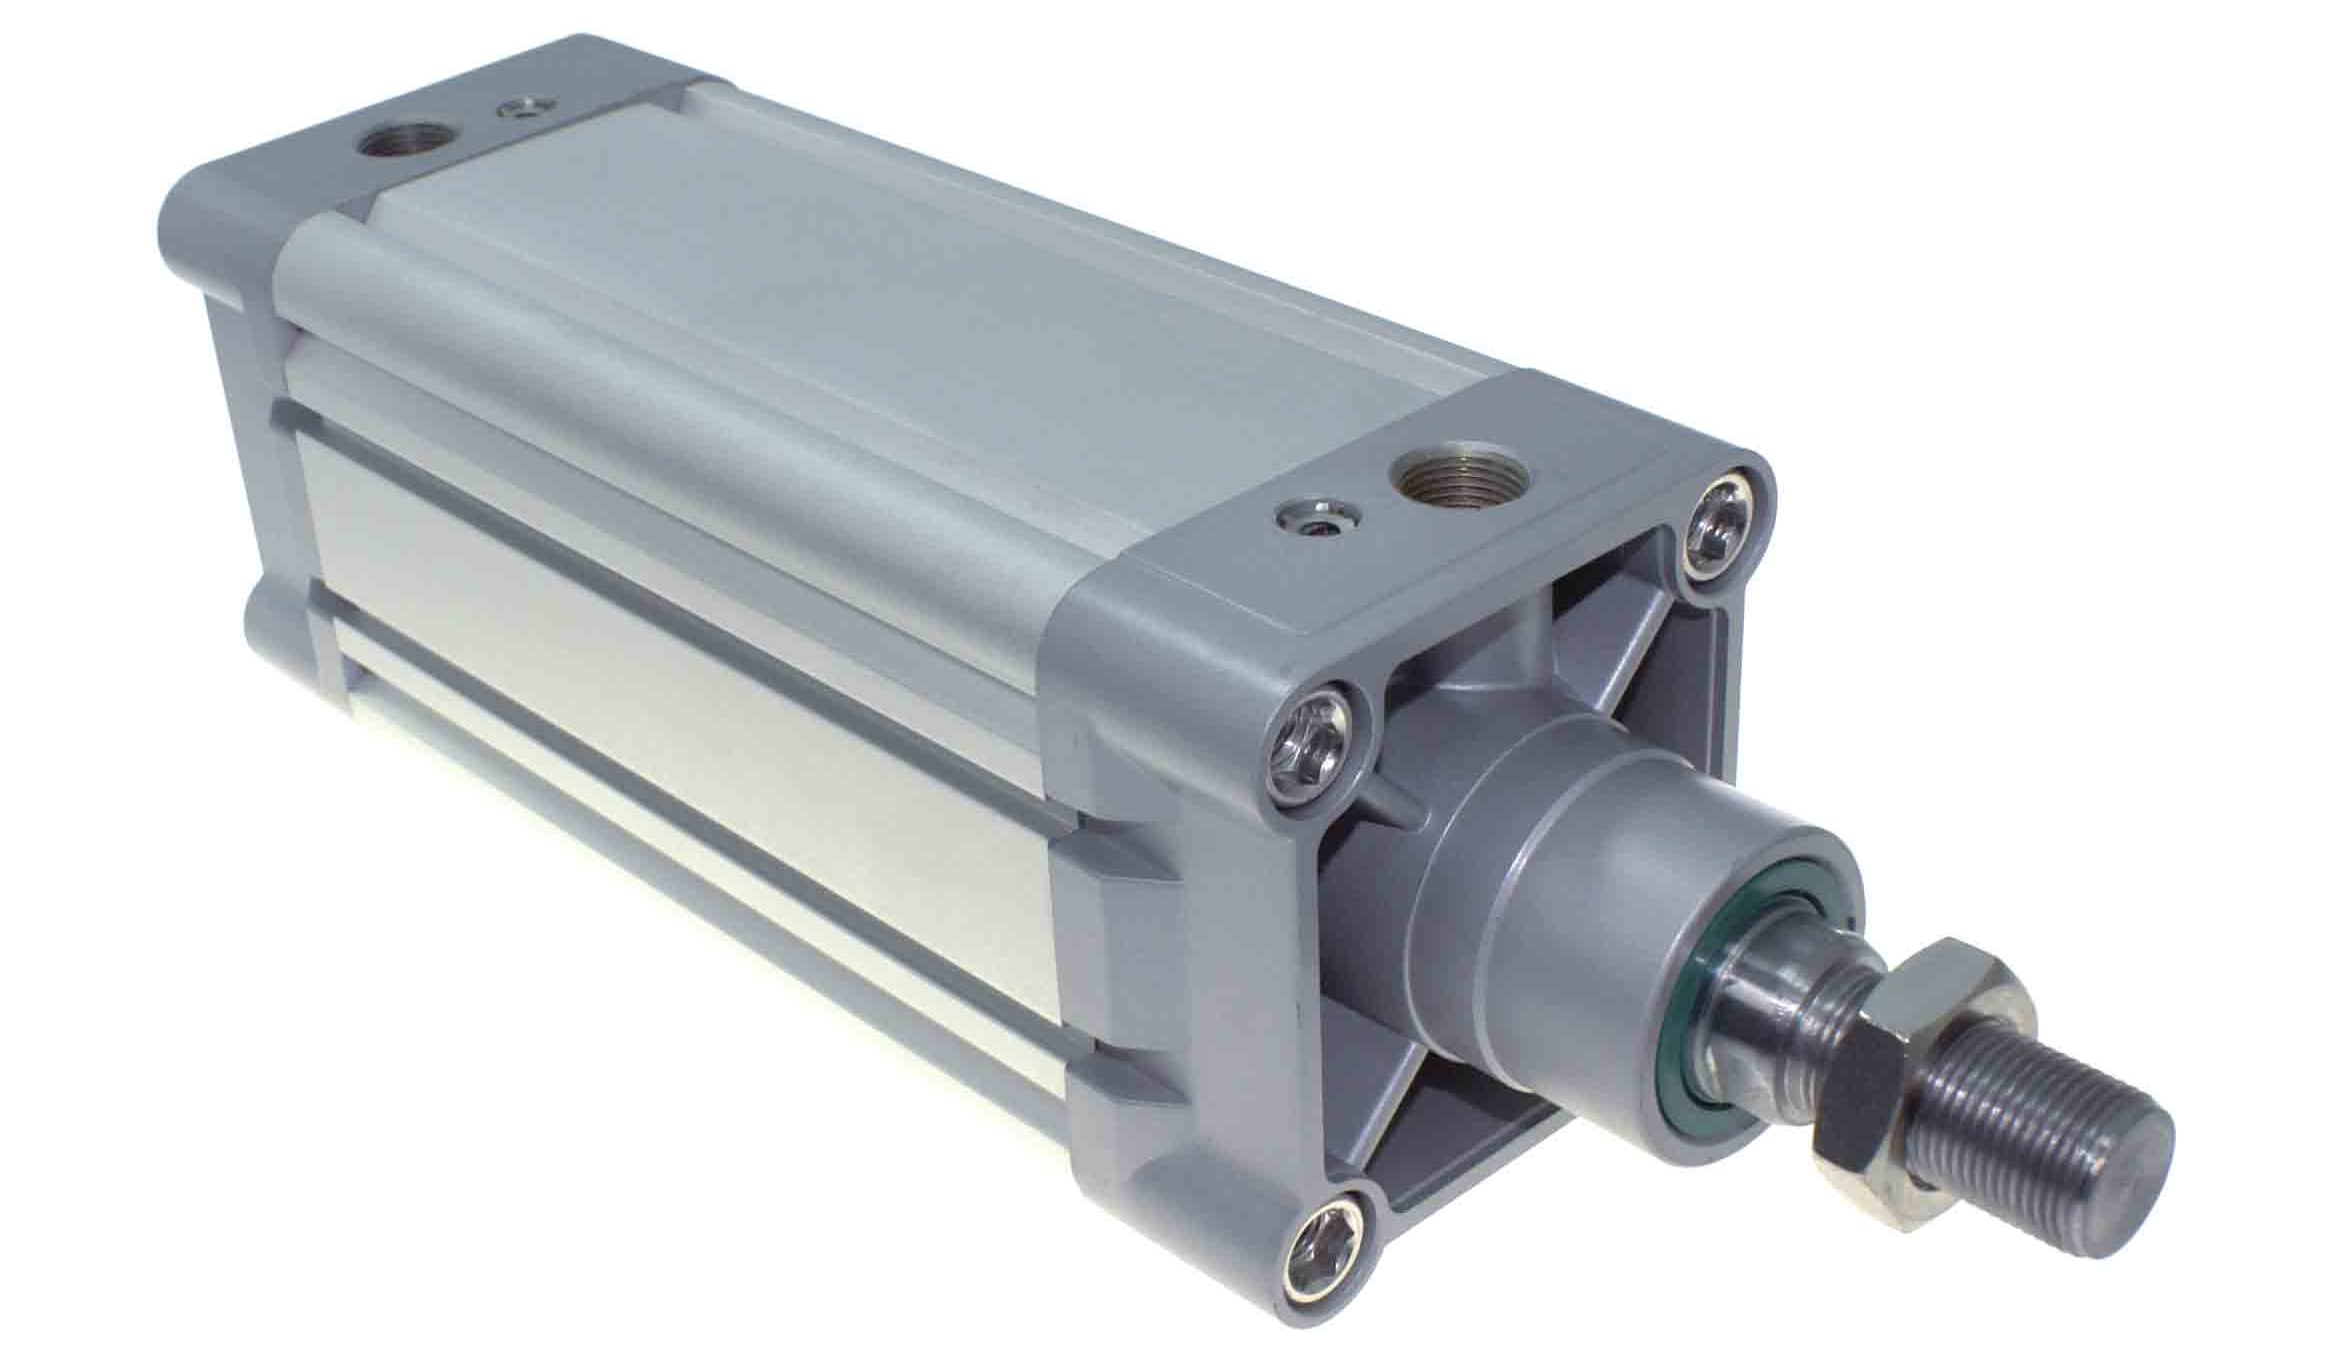
\includegraphics[width=1\linewidth]{Figuras/Ch14/fig33}
	\end{minipage}
	\hfill
	\begin{minipage}[c]{0.58\linewidth}
		\centering
		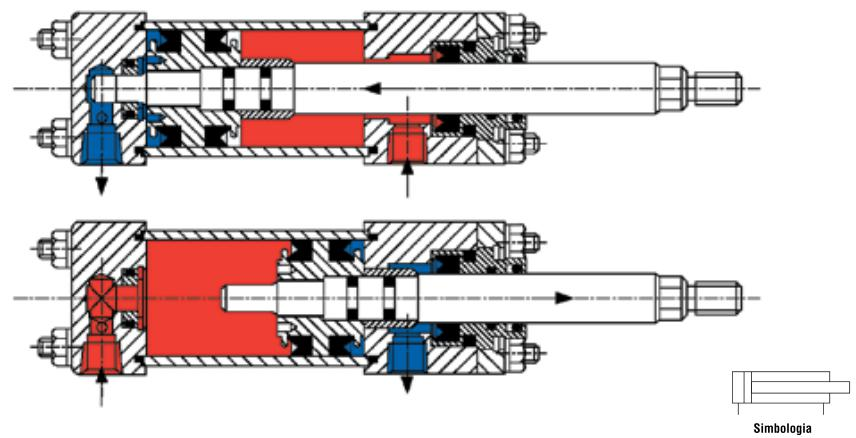
\includegraphics[width=1\linewidth]{Figuras/Ch14/fig34}
	\end{minipage}

\end{frame}


\begin{frame}{Elementos de trabalho - Atuadores pneumáticos}
	\begin{block}{Atuadores rotativos}
		\begin{itemize}
			\item Seu deslocamento é rotativo ao invés de linear.
		\end{itemize}
	\end{block}
	
	\medskip
	
	\centering
	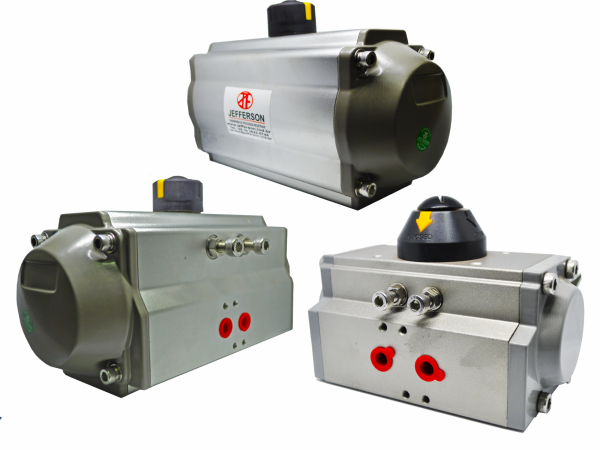
\includegraphics[width=0.6\linewidth]{Figuras/Ch14/fig39}
\end{frame}


\begin{frame}{Circuitos pneumáticos}
	\begin{block}{Introdução}
		\begin{itemize}
			\item Os circuitos pneumáticos podem ser vistos de forma análoga aos elétricos, embora hajam grandes diferenças estruturais.
		\end{itemize}
	\end{block}
	
	\medskip
	
	\centering
	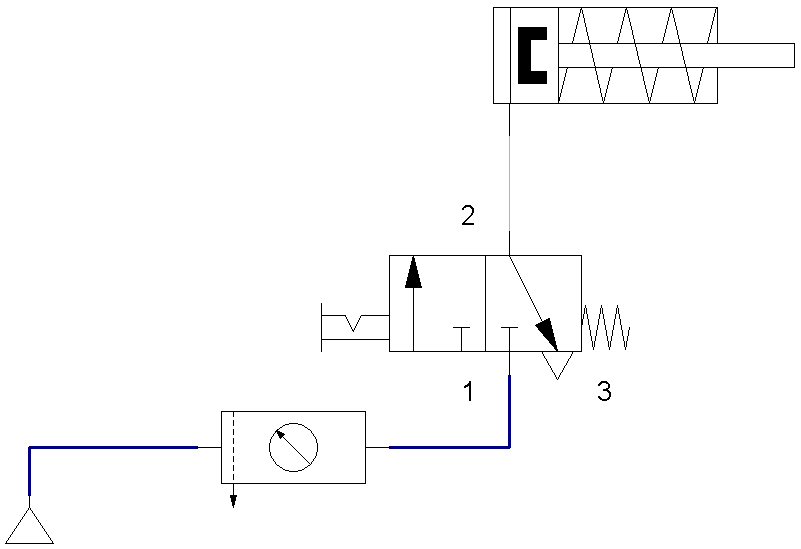
\includegraphics[width=0.55\linewidth]{Figuras/Ch14/fig40}
\end{frame}


\begin{frame}{Circuitos pneumáticos}
	\begin{block}{Observação}
		\begin{itemize}
			\item Os triângulos são representações de entradas e escapes de ar comprimido.
		\end{itemize}
	\end{block}
	
	\medskip
	
	\centering
	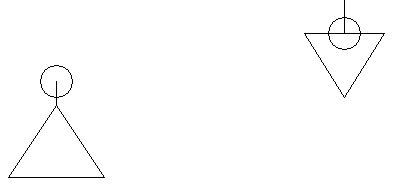
\includegraphics[width=0.8\linewidth]{Figuras/Ch14/fig41}
	
\end{frame}


\begin{frame}{Circuitos pneumáticos - Exemplo \#01}
	\begin{block}{}
		\begin{itemize}
			\item Neste circuito utilizou-se um cilindro de simples ação, bastando, para acioná-lo, usar uma válvula direcional manual de retorno por mola 3/2 vias.
		\end{itemize}
	\end{block}
	
	\medskip
	
	\centering
	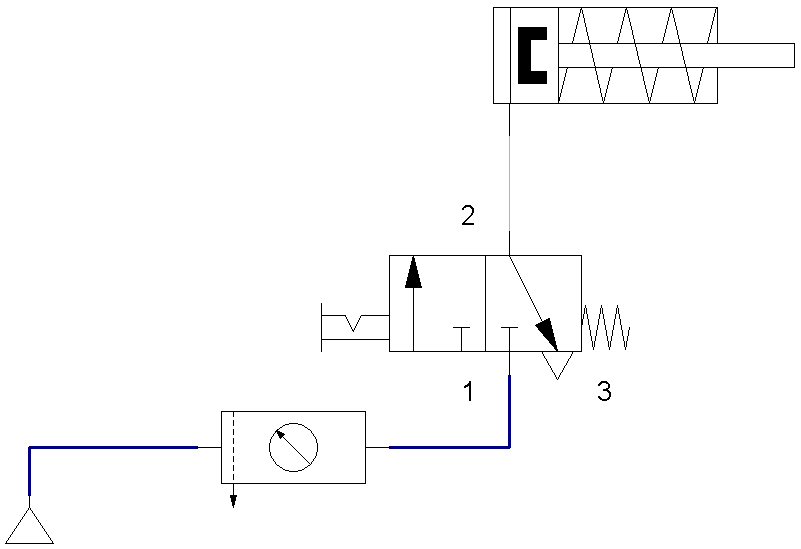
\includegraphics[width=0.65\linewidth]{Figuras/Ch14/fig40}
	
\end{frame}


\begin{frame}{Circuitos pneumáticos - Exemplo \#01}
	
	\centering
	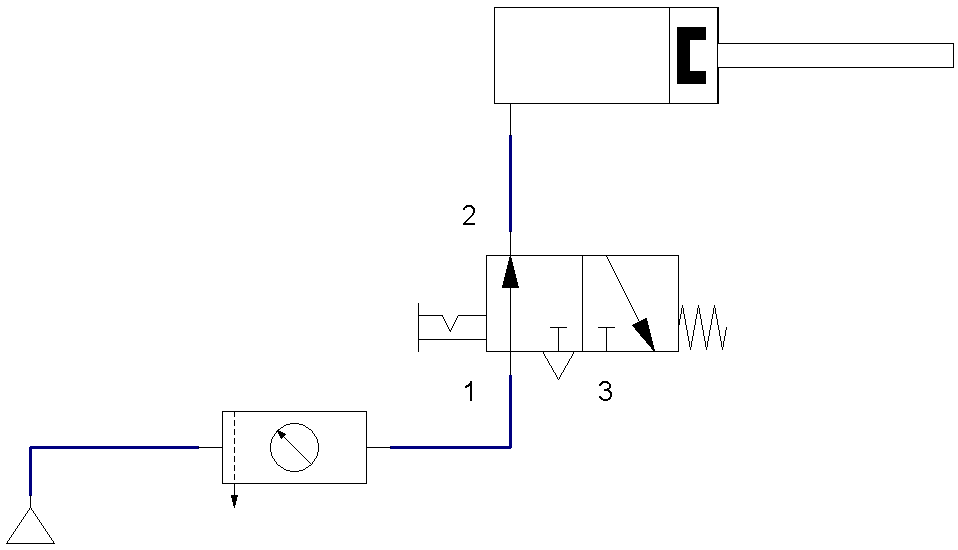
\includegraphics[width=0.9\linewidth]{Figuras/Ch14/fig40n2}
	
\end{frame}


\begin{frame}{Circuitos pneumáticos - Exemplo \#02}
	\begin{block}{}
		\begin{itemize}
			\item Caso desejemos utilizar um cilindro de dupla ação devemos utilizar no mínimo uma válvula de 4/2 vias, já que é necessário manusear o ar comprimido de ambos compartimentos do cilindro.
		\end{itemize}
	\end{block}
	
	\medskip
	
	\centering
	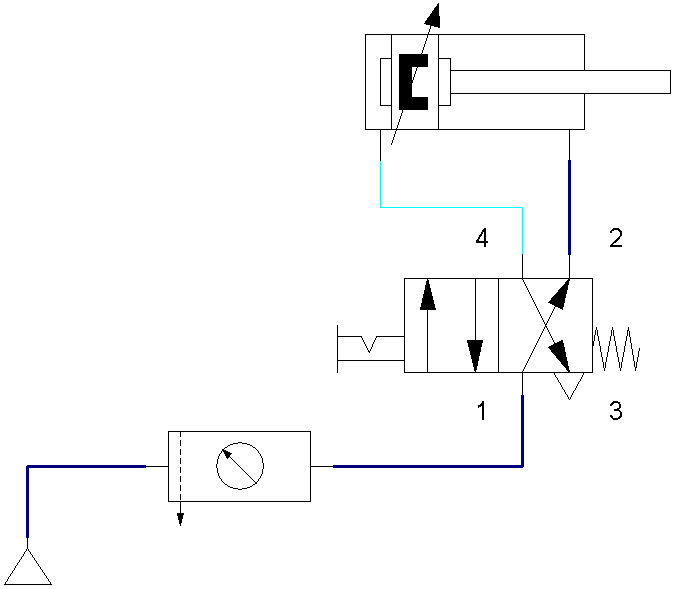
\includegraphics[width=0.55\linewidth]{Figuras/Ch14/fig42}
	
\end{frame}


\begin{frame}{Circuitos pneumáticos - Exemplo \#02}
	
	\centering
	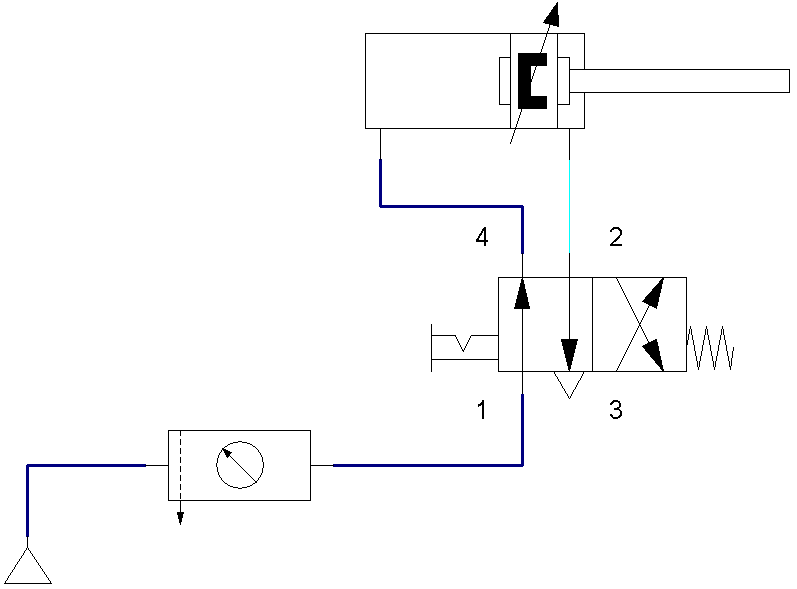
\includegraphics[width=0.8\linewidth]{Figuras/Ch14/fig42n2}
	
\end{frame}


\begin{frame}{Circuitos pneumáticos}
	\begin{block}{Automação}
		\begin{itemize}
			\item Podemos automatizar algumas operações de cilindros através de válvulas de fim de curso.
		\end{itemize}
	\end{block}
	
	\medskip
	
	\centering
	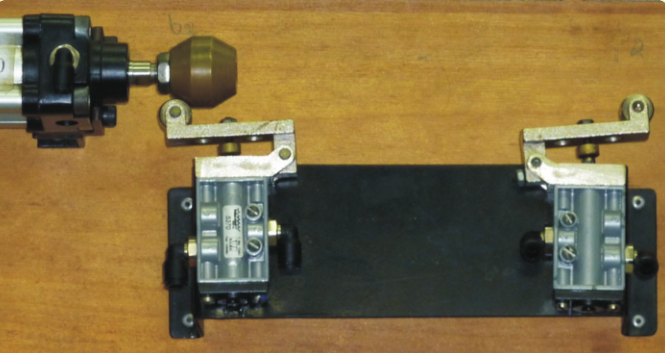
\includegraphics[width=0.8\linewidth]{Figuras/Ch14/fig43}
	
\end{frame}


\begin{frame}{Circuitos pneumáticos}
	\begin{block}{Automação}
		As válvulas de fim de curso são representadas no diagrama em \textbf{dois locais}:
		\begin{enumerate}
%			\setcounter{enumi}{1}
			\item No atuador onde se encontram \textbf{fisicamente}, representando onde, em seu curso, irão ser atuadas.
		\end{enumerate}
	\end{block}
	
	\medskip
	
	\centering
	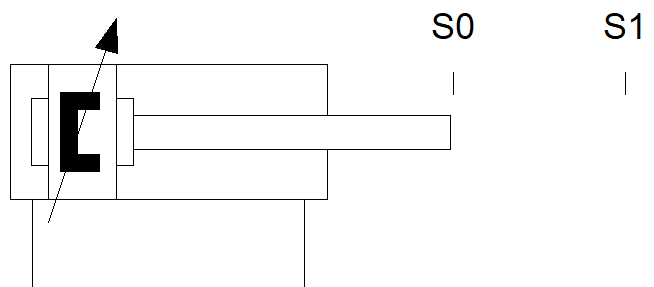
\includegraphics[width=0.8\linewidth]{Figuras/Ch14/fig45}
	
\end{frame}


\begin{frame}{Circuitos pneumáticos}
	\begin{block}{Automação}
		\begin{enumerate}
			\setcounter{enumi}{1}
			\item Na válvula onde irão atuar.
		\end{enumerate}
	\end{block}
	
	\medskip
	
	\centering
	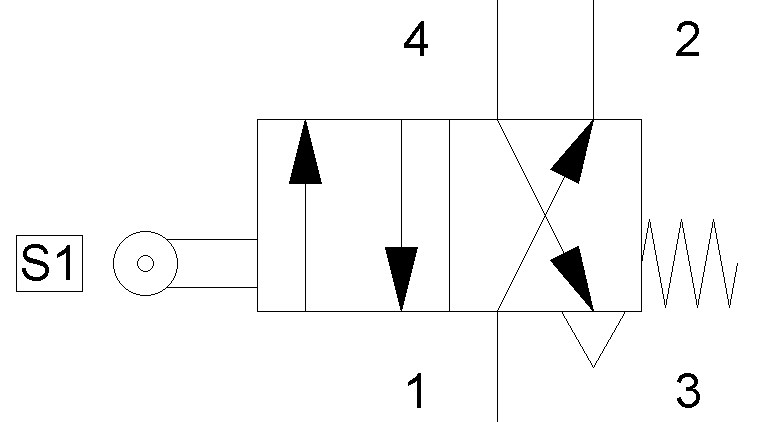
\includegraphics[width=0.8\linewidth]{Figuras/Ch14/fig46}
	
\end{frame}


\begin{frame}{Circuitos pneumáticos - Exemplo \#03}
	\begin{block}{}
		\begin{itemize}
			\item Na prática podemos fazer um cilindro de operação automática.
		\end{itemize}
	\end{block}
	
	\medskip
	
	\centering
	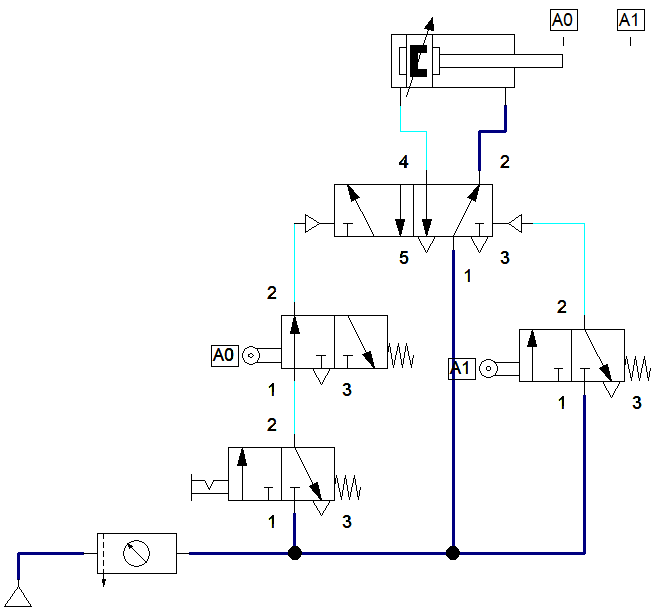
\includegraphics[height=0.7\textheight]{Figuras/Ch14/fig47}
	
\end{frame}


\begin{frame}{Circuitos pneumáticos - Exemplo \#03}
	
	\centering
	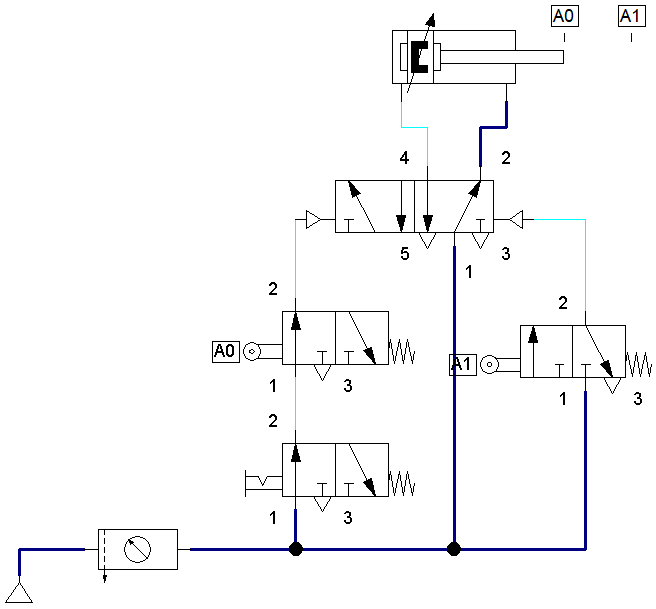
\includegraphics[width=0.7\linewidth]{Figuras/Ch14/fig47n2}
	
\end{frame}


\begin{frame}{Circuitos pneumáticos - Exemplo \#03}
	
	\centering
	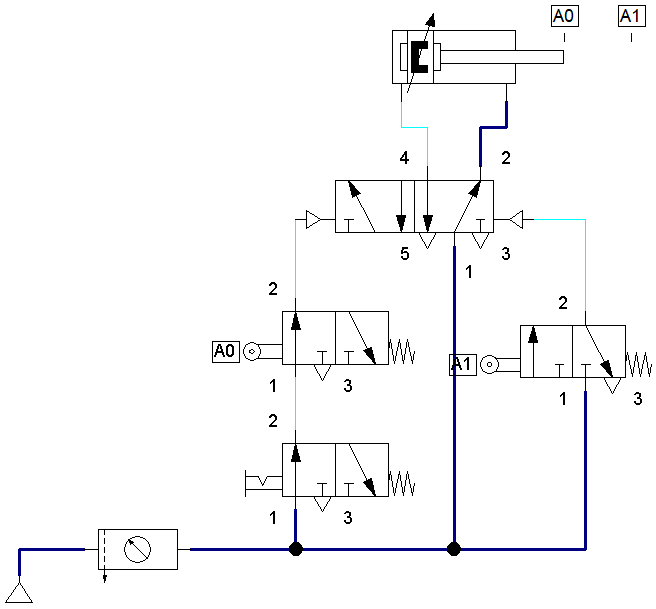
\includegraphics[width=0.7\linewidth]{Figuras/Ch14/fig47n2}
	
\end{frame}


\begin{frame}{Circuitos pneumáticos - Exemplo \#03}
	
	\centering
	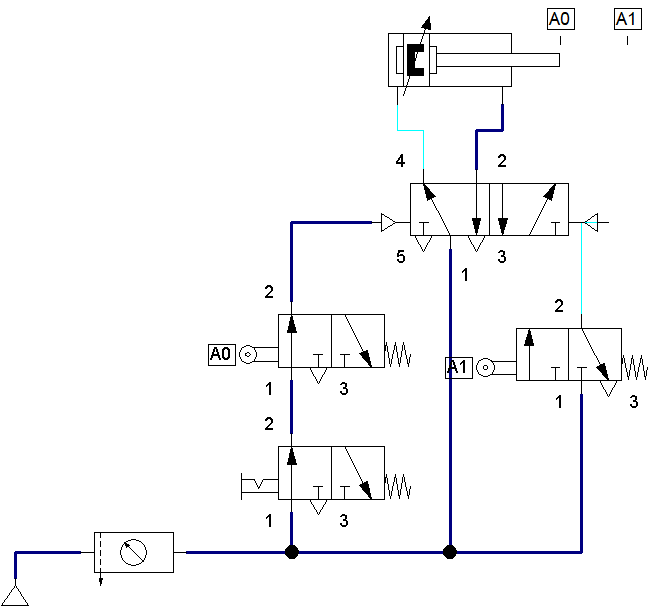
\includegraphics[width=0.7\linewidth]{Figuras/Ch14/fig47n3}
	
\end{frame}


\begin{frame}{Circuitos pneumáticos - Exemplo \#03}
	
	\centering
	\includegraphics[width=0.7\linewidth]{Figuras/Ch14/fig47n4}
	
\end{frame}


\begin{frame}{Circuitos pneumáticos - Exemplo \#03}
	
	\centering
	\includegraphics[width=0.7\linewidth]{Figuras/Ch14/fig47n5}
	
\end{frame}


\begin{frame}{Circuitos pneumáticos - Exemplo \#04}
	\begin{block}{}
		\begin{itemize}
			\item Nesse exemplo podemos controlar a \textbf{velocidade} de cada movimento através das \textbf{válvulas reguladoras de fluxo}.
		\end{itemize}
	\end{block}
	
	\medskip
	
	\centering
	\includegraphics[width=0.55\linewidth]{Figuras/Ch14/fig48}
	
\end{frame}


\begin{frame}{Circuitos pneumáticos - Exemplo \#05}
	
	\centering
	\includegraphics[width=0.8\linewidth]{Figuras/Ch14/fig48n2}
	
	\medskip
	
	Circuito com elemento OU
	
\end{frame}


\begin{frame}{Circuitos pneumáticos - Exemplo \#05}
	
	\centering
	\includegraphics[width=0.8\linewidth]{Figuras/Ch14/fig48n22}
	
\end{frame}


\begin{frame}{Circuitos pneumáticos - Exemplo \#05}
	
	\centering
	\includegraphics[width=0.8\linewidth]{Figuras/Ch14/fig48n23}
	
\end{frame}


\begin{frame}{Circuitos pneumáticos - Exemplo \#05}
	
	\centering
	\includegraphics[width=0.8\linewidth]{Figuras/Ch14/fig48n24}
	
\end{frame}


\begin{frame}{Circuitos pneumáticos - Exemplo \#06}
	
	\centering
	\includegraphics[width=0.8\linewidth]{Figuras/Ch14/fig48n3}
	
	\medskip
	
	Circuito com elemento E
	
\end{frame}


\begin{frame}{Circuitos pneumáticos - Exemplo \#06}
	
	\centering
	\includegraphics[width=0.8\linewidth]{Figuras/Ch14/fig48n32}
	
\end{frame}


\begin{frame}{Circuitos pneumáticos - Exemplo \#06}
	
	\centering
	\includegraphics[width=0.8\linewidth]{Figuras/Ch14/fig48n33}
	
\end{frame}


\begin{frame}{Circuitos pneumáticos - Exemplo \#06}
	
	\centering
	\includegraphics[width=0.8\linewidth]{Figuras/Ch14/fig48n34}
	
\end{frame}


\begin{frame}{Circuitos pneumáticos - Exemplo \#07}
	
	\centering
	\includegraphics[width=0.8\linewidth]{Figuras/Ch14/fig48n4}
	
	\medskip
	
	Circuito com ambos elementos lógicos
	
\end{frame}


\begin{frame}{Circuitos pneumáticos - Exemplo \#07}
	
	\centering
	\includegraphics[width=0.9\linewidth]{Figuras/Ch14/fig48n42}
	
\end{frame}


\begin{frame}{Circuitos pneumáticos - Exemplo \#07}
	
	\centering
	\includegraphics[width=0.9\linewidth]{Figuras/Ch14/fig48n43}
	
\end{frame}


\begin{frame}{Circuitos pneumáticos - Exemplo \#07}
	
	\centering
	\includegraphics[width=0.9\linewidth]{Figuras/Ch14/fig48n44}
	
\end{frame}


\begin{frame}{Circuitos pneumáticos - Exemplo \#08}
	\begin{block}{Comandos elétricos}
		\begin{itemize}
			\item Nos circuitos \textbf{eletropneumáticos} a parte mais complexa -- da lógica -- fica \textbf{separada} da parte de acionamentos pneumáticos.
		\end{itemize}
	\end{block}
	
	\medskip
	
	\begin{minipage}{0.48\linewidth}
		\centering
		\includegraphics[height=0.6\textheight]{Figuras/Ch14/fig49}
		\smallskip
		
		Circuito pneumático
	\end{minipage}
	\hfill
	\begin{minipage}{0.48\linewidth}
		\centering
		\includegraphics[height=0.6\textheight]{Figuras/Ch14/fig50}
		\smallskip
		
		Circuito elétrico de comando
	\end{minipage}
	
\end{frame}


\begin{frame}{Circuitos pneumáticos - Exemplo \#08}
	\begin{block}{Observação}
		\begin{itemize}
			\item Para simplificar o entendimento de certo circuito pneumático podemos utilizar \textbf{sinais} para indicar \textbf{movimento}.
			\item Digamos que o cilindro abaixo seja nomeado ``A'', para dizer que ele \textbf{avança} podemos denotar ``A+'', e para dizer que \textbf{recua}, ``A-''.
		\end{itemize}
	\end{block}
	
	\medskip
	
	\centering
	\includegraphics[height=0.55\textheight]{Figuras/Ch14/fig49n2}
	
\end{frame}


\begin{frame}{Circuitos pneumáticos - Exemplo \#08}
	
	\centering
	\includegraphics[width=0.9\linewidth]{Figuras/Ch14/fig49n3}
	
\end{frame}


\begin{frame}{Circuitos pneumáticos - Exemplo \#09}
	
	\medskip
	\centering
	
	\includegraphics[height=0.8\textheight]{Figuras/Ch14/fig51}
	
\end{frame}


\begin{frame}{Circuitos pneumáticos - Exemplo \#09}
	
	\centering
	\includegraphics[height=0.8\textheight]{Figuras/Ch14/fig51n2}
	
\end{frame}


\begin{frame}{Circuitos pneumáticos - Exemplo \#09}
	
	\centering
	\includegraphics[height=0.8\textheight]{Figuras/Ch14/fig51n3}
	
\end{frame}


\begin{frame}{Circuitos pneumáticos - Exemplo \#09}
	
	\centering
	\includegraphics[height=0.8\textheight]{Figuras/Ch14/fig51n4}
	
\end{frame}


\begin{frame}{Circuitos pneumáticos - Exemplo \#10}
	
	\medskip
	\centering
	
	\includegraphics[width=0.8\linewidth]{Figuras/Ch14/fig52}
	
\end{frame}


\begin{frame}{Circuitos pneumáticos - Exemplo \#10}
	
	\centering
	\includegraphics[width=0.8\linewidth]{Figuras/Ch14/fig52n2}
	
\end{frame}


\begin{frame}{Circuitos pneumáticos - Exemplo \#10}
	
	\centering
	\includegraphics[width=0.8\linewidth]{Figuras/Ch14/fig52n3}
	
\end{frame}


\begin{frame}{Circuitos pneumáticos - Exemplo \#10}
	
	\centering
	\includegraphics[width=0.8\linewidth]{Figuras/Ch14/fig52n4}
	
\end{frame}


\begin{frame}{Circuitos pneumáticos - Exemplo \#10}
	
	\centering
	\includegraphics[width=0.8\linewidth]{Figuras/Ch14/fig52n5}
	
\end{frame}


\frame{
	\frametitle{Exercícios}
	\begin{block}{}
		01. Em uma indústria automotiva existem dois cilindros, A e B, que encaixam uma roda, atuando simultaneamente. Monte um possível circuito para esse cenário.
	\end{block}
}

\section*{Referências}
\frame{
	\frametitle{Referências e Exercícios Complementares}
	\begin{itemize}
		\item MELCONIAN, Sarkis. Sistemas Fluidomecânicos - Hidráulica e Pneumática, 1 ed. Érica, 2014.
	\end{itemize}
	%\centering{\alert{Página 546 - \textbf{Capítulo 6}}} \\
	%\centering{\alert{Lista de exercícios 01}}
}
